
\section{FourShadow Microarchitecture}
\label{sec:design}

\subsection{Overview of the Extensions}
\label{sec:design_overview}

\begin{figure*}[ht]
    \centering
    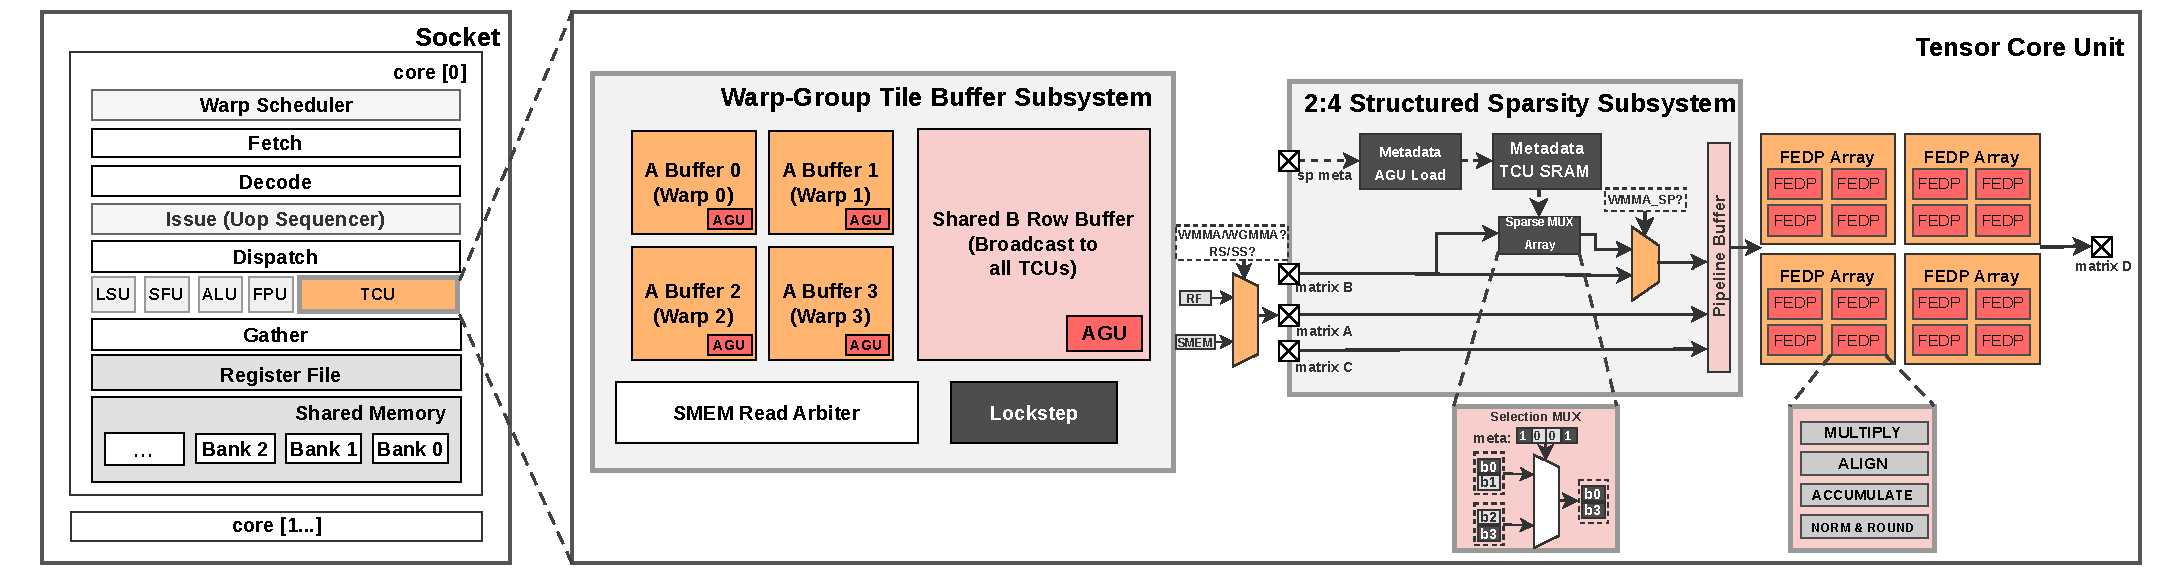
\includegraphics[width=\textwidth]{hpca2027-latex-template/fig/fourshadow_uarch.pdf}
    \caption{FourShadow's complete datapath highlighting its Warp-Group and Sparse Tensor Core Unit Extensions to a baseline Vortex GPGPU SIMT Core.}
    \label{fig:figure_integration}
\end{figure*}

FourShadow adds two extensions to the base tensor core of Section~\ref{sec:bg_tcu}; Figure~\ref{fig:figure_integration} shows the complete datapath with both. The warp-group tensor core (Section~\ref{sec:design_wgmma}) makes the warps of a warpgroup execute one matrix operation, one tensor block per warp, with operands read from shared memory through the Warp-Group Tile Buffer Subsystem: one private $A$ buffer per tensor block and one $B$ buffer shared by all blocks. The sparse tensor core (Section~\ref{sec:design_sparse}) adds 2:4 structured sparsity: a metadata SRAM in every tensor block and a Selection Mux Array that picks the $B$ elements matching the retained $A$ elements. Section~\ref{sec:design_pm} describes the programming model that selects among warp-level MMA, warp-group MMA and their sparse forms at compile time.

\subsection{Warp-group Tensor Core Extension}\label{para:wgmma}\label{sec:design_wgmma}
\subsubsection{Microarchitecture Design}

\begin{figure}
\small
\hrule
\vspace{3pt}
 
{\raggedright
\textit{Given:}\ $M,\,N,\,K,\,\mathit{NT},\,\mathit{NW},\,\mathit{NRC}$,\quad
$\rho=\tfrac{4}{\mathrm{sizeof}(\texttt{input\_dtype})}$\par
\textit{Standard WGMMA:}\ $\mathit{fedpK}=\mathit{tcK}$\par}
 
\centering
\textbf{\textsc{WGMMA tile (per-warp work chunk)}}
\begin{flalign}
&\mathit{xtileM}_{\mathrm{wg}} = 2\mathit{tcM},\quad
\mathit{xtileK}_{\mathrm{wg}} = 2\mathit{tcK} & \\
&\mathit{tileK}_{\mathrm{wg}}
 = \mathit{xtileK}_{\mathrm{wg}}\rho
 = 2\mathit{tcK}\rho & \\
&\mathit{xtileN}_{\mathrm{wg}}
 = \tfrac{\mathit{NRC}\times\mathit{NT}}
         {\mathit{xtileM}_{\mathrm{wg}}}
 = \tfrac{\mathit{NRC}\times\mathit{NT}}
         {2\mathit{tcM}} &
\end{flalign}
 
\noindent
\textbf{\textsc{WGMMA steps (micro-ops per warp)}} 
\begin{flalign}
&m_{\mathrm{steps}}
 = \tfrac{\mathit{xtileM}_{\mathrm{wg}}}{\mathit{tcM}}
 = 2 & \\
&n_{\mathrm{steps}}
 = \tfrac{\mathit{xtileN}_{\mathrm{wg}}}{\mathit{tcN}}
 = \tfrac{\mathit{NRC}\times\mathit{NT}}
         {2\mathit{tcM}\mathit{tcN}}
 = \tfrac{\mathit{NRC}}{2} & \\
&k_{\mathrm{steps}}
 = \tfrac{\mathit{xtileK}_{\mathrm{wg}}}{\mathit{fedpK}}
 = 2 &
\end{flalign}
 
\hrule
\vspace{3pt}
 
\noindent
\textbf{\textsc{Warp-group tile}}
\begin{flalign}
&\mathit{wgTileM}
 = \mathit{NW}\times\mathit{xtileM}_{\mathrm{wg}}
 = 2\mathit{NW}\mathit{tcM} & \\
&\mathit{wgTileN}
 = \mathit{xtileN}_{\mathrm{wg}} & \\
&\mathit{wgTileK}
 = \mathit{tileK}_{\mathrm{wg}}
 = 2\mathit{tcK}\rho &
\end{flalign}
 
\noindent
\textbf{\textsc{Warp indexing and tile ownership}}
\begin{flalign}
&0 \leq w < \mathit{NW} & \\
&M_w = M_{\mathrm{CTA}} + w\mathit{xtileM}_{\mathrm{wg}} & \\
&N_w = N_{\mathrm{CTA}},\quad
K_w = K_{\mathrm{tile}} & \\
&A^{(w)}
 = A[M_w:M_w+\mathit{xtileM}_{\mathrm{wg}},\,
     K_w:K_w+\mathit{tileK}_{\mathrm{wg}}] & \\
&B^{(\mathrm{wg})}
 = B[K_w:K_w+\mathit{tileK}_{\mathrm{wg}},\,
     N_w:N_w+\mathit{xtileN}_{\mathrm{wg}}] & \\
&C^{(w)}
 = C[M_w:M_w+\mathit{xtileM}_{\mathrm{wg}},\,
     N_w:N_w+\mathit{xtileN}_{\mathrm{wg}}] &
\end{flalign} 
\hrule
 
\caption{WGMMA warp-group tiling, indexing, and micro-op decomposition. Each synchronized
uop round dispatches the same \((m,n,k)\) coordinate to \(\mathit{NW}\) TCU
blocks; warp \(w\) supplies its own A rows while all warps consume the same
B tile.}
\label{fig:wgmma_tiling_equations}
\end{figure}

\textbf{Warp-group formation.} WGMMA groups a fixed number of warps, set by the configured issue width, into one cooperative unit. Each warp is indexed along the M-dimension of the warp-group tile. With $\mathit{NW}$ warps per warp-group, $\mathit{NW}$ A-tiles of size $M{\times}K$ are loaded, one per warp, and all warps share a single B-tile of size $WK{\times}N$. Each WGMMA instruction produces one $WM{\times}N$ output C tile. Raising the number of accumulator registers (NRC) to 2x (16) or 4x (32) extends the number of uop iterations in the N-dimension, producing a $WK{\times}2N$ or $WK{\times}4N$ output tile instead. The full set of tiling, indexing, and micro-op equations for the WGMMA-extended TCU is given in Fig.~\ref{fig:wgmma_tiling_equations}.

\textbf{Tensor block organization.} With $NT=32$ and $\mathrm{ISSUE\_WIDTH}=4$, the core instantiates four tensor blocks, each built from the same 32-cell, $8\times4$ FEDP array used in the baseline TCU. Fig.~\ref{fig:figure_integration} shows the corresponding microarchitecture: the Warp-Group Tile Buffer Subsystem adds four private A buffers and one shared B row buffer alongside the existing FEDP arrays. Issue width sets how many of these blocks exist, and therefore how many warps of the warp-group can be serviced in parallel; the FEDP count per block does not change. Each block accepts one micro-op from one warp. The four blocks do not split a single warp's operation between them: each processes one full warp from the group, all four consuming the same B tile while operating on disjoint A row stripes. This extends the matrix operation in the M dimension only. The row/column/depth mapping and the resulting dot product performed by cell $(i,j)$ in block $b$ are given in Fig.~\ref{fig:wgmma_tiling_equations}. Because every block needs the same K coordinates to compute its own output row from the shared B columns, warp-group formation extends M from 16 rows per warp to 64 rows per warp-group without changing $m_{\mathrm{steps}}=2$ or $k_{\mathrm{steps}}=2$: four parallel row stripes are added, not the depth needed to cover a $K=16$ tile.

\textbf{Number of accumulator registers (NRC).} Each WGMMA instruction expands into an ordered sequence of tensor micro-ops, with $m$ changing fastest, then $n$, then $k$ (Fig.~\ref{fig:wgmma_tiling_equations}). The two $m$ coordinates are issued back to back because both consume the same $B(k,n)$ block; only the private A row selection changes between them. NRC sets the number of 4-column tensor blocks covered in the N dimension, so $n_{\mathrm{steps}}=\mathrm{NRC}/2$:
\[
\begin{array}{c|c|c|c}
\mathrm{NRC} & n_{\mathrm{steps}} & \text{warp-group tile} & \text{uops/warp} \\ \hline
8  & 4  & 64\times16\times16 & 16\\
16 & 8  & 64\times32\times16 & 32\\
32 & 16 & 64\times64\times16 & 64
\end{array}
\]
When all four warp-group members progress together these become 16, 32, or 64 issue rounds, each performing four physical $8\times4\times8$ tensor operations, one per block, for a total of 64, 128, or 256 physical micro-ops. Each lane owns two accumulator registers per $n$ coordinate, one per $m$ coordinate, selected as $2n+m$; across 32 lanes this register set holds the complete $8\times4$ output block. NRC $=32$ is available only in SS mode, since RS mode reserves eight registers for the A fragment and leaves less register space for accumulators.

\textbf{Execution ordering.} Three separate mechanisms govern correctness. They are not a single cycle-accurate four-warp barrier. First, per-instruction sequencing: the first micro-op of a WGMMA instruction acquires the tensor execution path, intermediate micro-ops hold it, and the last releases it, so another tensor instruction cannot interleave mid-sequence. The scoreboard tracks the accumulator register dependencies in parallel. Second, CTA ownership: each tensor block records whether it is mid-sequence and which CTA owns it. Once any block enters a sequence, no warp from another CTA may begin conflicting WGMMA work while the current CTA still owns active blocks, though warps from the owning CTA remain free to occupy other blocks. Issue scheduling, refills, or backpressure can still skew the four warps relative to each other; correctness follows from retaining CTA ownership until the last micro-ops depart, not from lockstep execution. Third, shared-operand protection: the lowest-numbered active block supplies a B-tile key (descriptor, $k$, $n$, accumulator configuration); every other active block must match that key before consuming the shared B buffer, or it is backpressured. Skew between warp-group members is tolerated only when it cannot cause a block to read the wrong shared operand. Readiness for a compute micro-op and the sequence coordinate $q$ are given in Fig.~\ref{fig:wgmma_tiling_equations}; descriptor-setup micro-ops do not touch matrix data and skip tile-residency checks.

\textbf{Descriptor capture and RS/SS modes.} WGMMA reaches shared-memory operands through compact descriptors carrying a tile base and layout stride, captured either by an explicit setup op or by the first compute micro-op. A zero stride is a block-major layout, where an operand block lines up directly with a shared-memory bank row; a nonzero stride is row-major or K-major and forces the refill logic to gather rows into the internal tensor layout. The first compute micro-op always forces a fresh residency check and refill, even if its descriptor numerically matches the preceding instruction, because the kernel can overwrite the same shared-memory addresses between outer-K iterations; descriptor equality alone cannot guarantee the buffered data is current. In shared-memory/shared-memory (SS) mode, both A and B come from shared memory. In register/shared-memory (RS) mode, A comes from a fixed register fragment and bypasses the A-tile buffers, while B still uses the shared buffer. The FEDP array sees the same internal vector representation either way; only the source feeding A changes.

\textbf{Shared-memory tile buffering.} The kernel stages global-memory tiles into shared memory over the normal SIMT path, and CTA synchronization makes the writes visible to the tensor reads. Rather than issuing 32 independent lane loads per micro-op, the tensor subsystem uses a dedicated bank-parallel local-memory port (Fig.~\ref{fig:figure_integration}) that pulls a full bank row into an operand buffer per request; nonzero-stride layouts may need multiple requests to gather and reorder rows. This port shares physical banks with ordinary local-memory traffic through the same arbitration fabric. Five clients contend for it: four private A buffers, one per tensor block, and one shared B buffer, arbitrated five-to-one, each retaining independent residency state. Each private A buffer holds the current K stripe for its warp and both $m$ blocks, so the two $m$ micro-ops read different halves of the resident tile without a new shared-memory access; a refill is only needed when $k$, the descriptor, or the freshness state changes. The shared B buffer holds the current $B(k,n)$ block and broadcasts it structurally to all four blocks; its key excludes $m$ since both $m$ micro-ops need the same B data, so one $B(k,n)$ refill serves eight physical tensor operations, two $m$ coordinates across four warps. This is why B lives in one shared buffer instead of four private copies.

\textbf{Feeding the FEDP array.} Once operands are resident, the A buffer supplies eight row vectors for the current $m$, one per FEDP-array row, and the B buffer supplies four column vectors for the current $n$, one per FEDP-array column; the Cartesian product of these feeds all 32 FEDP cells. Each 32-bit operand word packs two FP16 elements, so four packed words supply the eight scalar elements needed for one 8-deep dot product. The accumulator read and write for each micro-op is selected by $2n+m$. Operand vectors, accumulator values, arithmetic format, and instruction identity move through the pipeline together, and a result-tracking queue carries warp, destination, lane, and instruction metadata through the arithmetic latency so backpressure cannot mismatch a result with the wrong micro-op. Each of the four tensor blocks has its own completion path back to the register file, even though all four share the B operand subsystem.

\textbf{Configurability.} Issue width sets how many tensor blocks exist and hence how many warp-group row stripes can advance concurrently. Thread count sets the FEDP-cell count and warp-level microtile shape. NRC extends N coverage through additional accumulator blocks. SS versus RS mode changes where A comes from and how much register space is left for accumulators. Element width sets packing density and bank-row utilization. The design keeps what benefits from independence, private A state, arithmetic pipelines, result tracking, commit, separate per block, while sharing what is mathematically common to the group: B-tile storage, descriptor consistency, and CTA ownership. This is what lets four warps behave as one 64-row matrix operation without a rigid cycle-by-cycle barrier between their schedulers.

\subsubsection{Design-Space Exploration}
 
Building on the warp-group MMA architecture above, we explore two design-space extensions that push WGMMA throughput and efficiency further: a wider FEDP dot-product unit, and moving WGMMA's descriptor load off the register file.
 
\textbf{2K-Wide FEDP.} FEDP dot-product length, the number of element pairs reduced per micro-op in the K-dimension, was previously capped by the register file, since all A and B tiles had to be staged there. WGMMA removes that constraint by sourcing operands directly from shared memory, so we double the FEDP length and halve the number of uop-steps needed in the K-dimension, as shown in Fig.~\ref{fig:fedp2k_blocks}.
 
\begin{figure}
    \centering
    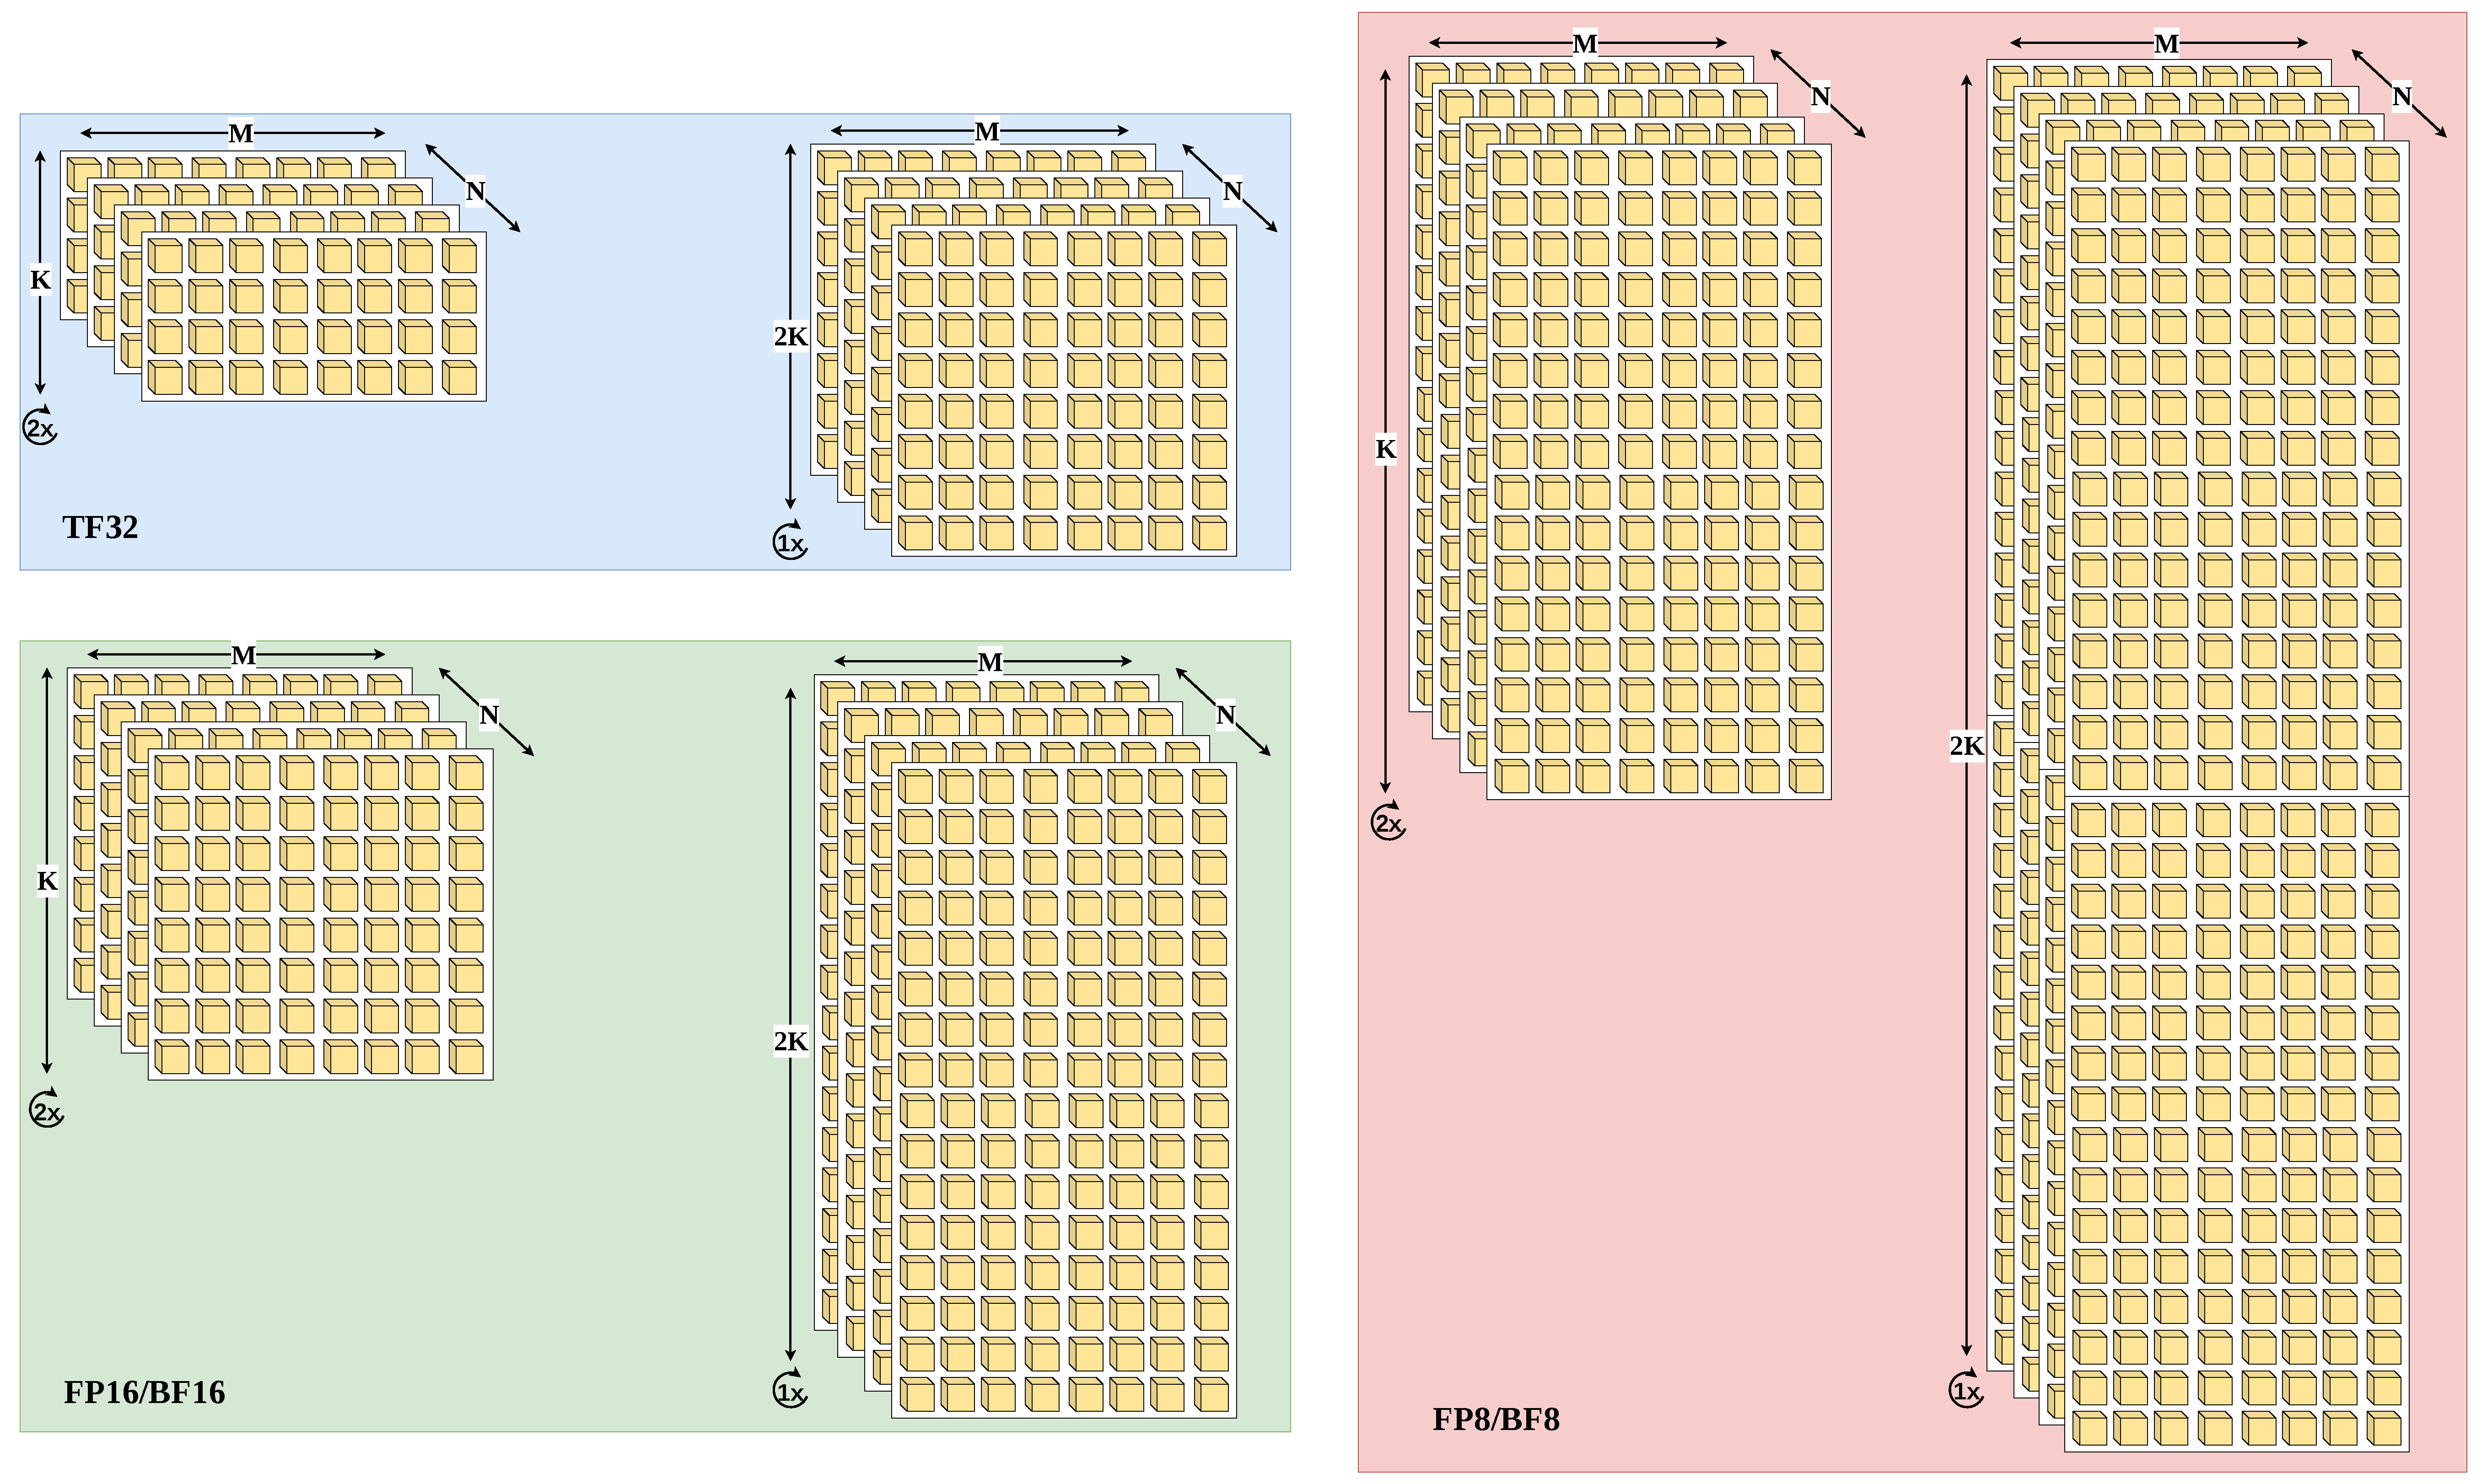
\includegraphics[width=0.8\linewidth]{hpca2027-latex-template/fig/fedp2k.pdf}
    \caption{Logical K vs 2K-Wide FEDP}
    \label{fig:fedp2k_blocks}
\end{figure}
 
In SS mode this change was straightforward: the Ten-Four FEDP microarchitecture already supports a configurable dot-product length, and both A and B come from SMEM. As before, WGMMA's rs1/rs2 fields load the A and B descriptors into x10/x11 on the first descriptor-setup-plus-compute micro-op, and every following micro-op keeps pulling from SMEM.
 
\textbf{Feeding 2K-Wide FEDP in RS Mode.} RS mode is less straightforward. 2K-Wide FEDP needs twice the A-tile operands from the register file, but rs2 is still needed to carry the B descriptor into x11. Our first attempt gave rs1 an implicit adjacent register pair, but this adds hidden source-register dependencies to the scoreboard and grows the operand collector, too expensive a change to the existing SIMT frontend, so we dropped it. Instead, when 2K-Wide FEDP is enabled in RS mode, we add one setup uop that only transfers the B descriptor to x11 via rs2; every following compute uop then reads tile A from both register fields, lower half from rs1, upper half from rs2. This extra setup uop adds under 1\% to end-to-end cycle count.
 
\textbf{Backward Compatibility with WMMA.} With 2K-Wide FEDP enabled, legacy WMMA instructions still need to execute correctly, but we cannot source their operands' extra "upper half" from the register file. We hardwire that upper half to zero for both A and B, which preserves existing WMMA micro-op semantics unchanged. We suspect NVIDIA does something similar in Hopper \cite{nvidia2022hopper}, evidenced by legacy WMMA there reaching only 62.9\% of theoretical peak throughput on average \cite{luo2025dissectingnvidiahopperarchitecture}. When 2:4 structured sparsity is also enabled, K-dimension uops are halved again; with both sparsity and 2K-Wide FEDP active, the uop count in K bottoms out at one, and the same zero-hardwiring keeps the FEDP inputs full.
 
\textbf{Pipeline Latency Tradeoff.} The baseline Ten-Four FEDP multiplies and reduces k-element pairs in a 4-stage pipeline. Doubling FEDP width to process 2x the elements adds critical-path latency in two places: \texttt{MULTIPLY}, from higher fanout on the shared operand, and \texttt{ACCUMULATE}, from twice the products to reduce, which adds an extra intermediate reduction row even with a 4:2 compressor-based carry-save adder tree. At smaller thread counts (NT=4, 8) this is manageable, but at larger thread counts (NT=16, 32) the FEDP pipeline needs more stages, and WMMA/WGMMA cycle latency grows with it. We also evaluate an 8-cycle-latency variant in the evaluation section below. Even with deeper pipelining this should still be a net throughput win: WMMA/WGMMA micro-ops are heavily pipelined already and can fill a deeper pipeline without stalling, especially for larger SGEMM kernels. NVIDIA appears to be making a similar move in the upcoming Rubin tcgen06 Tensor Cores \cite{nvidia2026rubin}.
 
\textbf{Why Not 4K or 8K-Wide?} We stop at 2K-wide for three reasons: (i) every FEDP unit becomes far more expensive, with significant fanout across the datapath; (ii) it sits heavily underutilized on WMMA and WMMA\_SPARSE instructions; (iii) it only yields marginally larger gains, and only at very large SGEMM kernel dimensions. Widening the core this way also erodes the programmability that inner-dot-product tensor cores exist to provide over rigid systolic arrays: fine-grained MMA hardware that handles irregular, any-dimension, and sparse workloads well.
 
\textbf{Descriptor Load Location.} Another experiment we perform moves WGMMA's A/B shared-memory descriptors out of the instruction's register operands and into a per-warp TCU SRAM, using the same transport path as sparsity metadata. Each warp first writes its 32-bit descriptors to shared memory, synchronizes, and issues one or two TCU\_LD instructions targeting the reserved f24/f25 slots. A TCU-side AGU then fetches those values through the LSU and deposits them into the warp's TCU SRAM space; subsequent WGMMA compute-uop expansion reads descriptors from there instead of the current x10/x11 integer registers. The goal is to relieve register-file pressure, especially with 2K-Wide FEDP enabled. The tradeoff is that descriptor setup in TCU SRAM now costs a shared-memory store, a CTA barrier, LSU traffic, scoreboard/writeback activity, and serialized AGU transactions, all before any matrix work begins, for just one or two 32-bit values.

\subsection{Sparse Tensor Core Extension}\label{sec:design_sparse}

\textbf{Analytic Speedup Model.}
Figure~\ref{fig:sparse_analytic} captures an analytic model of the speedup derived from adding a 2:4 structure sparsity subsystem to the TCU. The dense cost is normalized to~1 and sparsity halves the compute term~$\mathit{TC}$ but adds metadata overhead $\mathit{MO}$ that grows linearly as the input datatype narrows.

\begin{figure}[ht]
\small
\raggedright
\hrule
\vspace{3pt}
\noindent\textbf{Dense (normalized to 1):}
\begin{equation}
\mathit{Cycle}_{\text{dense}} = A_{\text{load}} + B_{\text{load}} + \mathit{TC} + D_{\text{store}} = 1
\end{equation}
\noindent\textbf{Sparse:}
\begin{equation}
\mathit{Cycle}_{\text{sparse}} = A_{\text{load}} \!\times\! s_{\text{eff}} + B_{\text{load}} + \tfrac{1}{2}\,\mathit{TC} + D_{\text{store}}
\end{equation}
\noindent\textbf{Speedup and effective saving:}
\begin{equation}
\mathit{Speedup} = \frac{1}{\mathit{Cycle}_{\text{sparse}}}, \qquad
s_{\text{eff}} = 1 - \tfrac{1}{2} + \mathit{MO}
\end{equation}
\noindent where $\mathit{MO}$ is the metadata overhead relative to matrix~$A$:
\begin{equation}
\mathit{MO} = \frac{\texttt{sizeof}(\texttt{input\_dtype})}{32}
= \begin{cases} 3.125\% & \texttt{tf32} \\ 6.25\% & \texttt{fp16/bf16} \\ 12.5\% & \texttt{fp8/bf8} \end{cases}
\end{equation}
\hrule
\caption{Analytic speedup model of sparse TCU over dense TCU. (Assume the matrix C is initialized as zero)}
\label{fig:sparse_analytic}
\end{figure}


\textbf{Sparse Metadata Flow.} One of the main modifications to the TCU microarchitecture here is the addition of the metadata operand inputs. Metadata has different lifetime and reuse properties than $A$ and $B$, so it moves through a separate path. Before sparse execution, the kernel issues \texttt{load\_sp\_metadata}: each participating lane contributes one 32-bit metadata word, and a warp-level address generator forms the load as an ordinary load/store-scheduler request rather than a tensor tile-buffer fetch, so metadata can live in either global or local memory. The returned lane words are assembled into a warp metadata record and written identically into every tensor block's metadata SRAM, indexed by warp identity with subregions selected by the current $m$ and $k$ coordinates. Replication means any issue path can run that warp's sparse micro-ops, rather than tying the warp to whichever block happened to complete its metadata load. A scoreboard dependency orders the two operations: the metadata load produces a reserved token, and sparse execution consumes it, so sparse micro-ops cannot issue until the load returns and its SRAM write completes. This removes the need for a separate software-visible metadata fence.

\textbf{Sparse FEDP Selection.} The compressed $A$ values are sent directly to the FEDP inputs; the hardware does not reconstruct a dense vector by inserting zeros. Instead, the row-specific metadata drives the Selection Mux Array as a gather network on the $B$ side, selecting the two $B$ elements that match the two retained $A$ positions for each group of four. This selector is replicated across the FEDP grid because metadata is row-dependent: different $A$ rows can retain different positions even though the underlying $B$ candidates are shared. A sparse micro-operation still performs eight nonzero products per output element, but those products now cover sixteen logical $K$ positions instead of eight, so sparse execution needs only half as many $k\_steps$ as dense execution for the same tile.

\textbf{Asymmetric vs.\ Symmetric Configurations.} Enabling 2:4 sparsity halves matrix~$A$'s $K$ dimension, reducing both load volume and MMA micro-ops ($k\_steps$ halved) at the cost of metadata. The $B$ operand preparation, however, differs fundamentally between asymmetric and symmetric configurations, and the performance benefit applies only to the asymmetric group ($\mathit{NT}{\in}\{2,8,32\}$).

Figure~\ref{fig:figure_register_mapping}(a) shows the $\mathit{NT}{=}8$ case. In the dense baseline (green), \texttt{reg0} of matrix~$B$ holds two horizontally packed sub-blocks, each filling half the register. With sparsity enabled (red), each compressed $A$ row must pair with two candidate $B$ columns for metadata-driven selection, changing the $B$ layout to vertical column pairs (``$\times$2 col candidates''). Because the asymmetric layout already half-utilizes each register, this rearrangement fits naturally within the existing width. As shown in the red annotations, $\mathit{xtileK}$ halves from 8 to 4, reducing $k\_steps$ from 4 to 2 while all FEDP units remain fully active.

The symmetric case in Figure~\ref{fig:figure_register_mapping}(b) with $\mathit{NT}{=}4$ faces a structural constraint. In the dense baseline (green), each $B$ block of $\mathit{tcK}{\times}\mathit{tcN} = 2{\times}2 = 4$ already fills the entire \texttt{reg0}. Doubling the $B$ columns for sparsity would require a fifth source operand, but FourShadow's datapath, inherited from Vortex's R4-type \texttt{fmadd} path, supplies exactly four register fields, all occupied by the micro-op encoding for $A$, $B$, $C$, and $D$. Instead, as shown in the red annotations, we halve $\mathit{tcN}$ from 2 to 1, doubling $n\_steps$ from 2 to 4. Although $k\_steps$ halves from 2 to 1, the total micro-op count remains 16, with only half the FEDP units active per micro-op, alternating via thread masks. Consequently, the symmetric group achieves barely any speedup from sparsity, but FourShadow preserves full configurability across all thread counts.

\subsection{Programming Model}
\begin{figure}
    \centering
    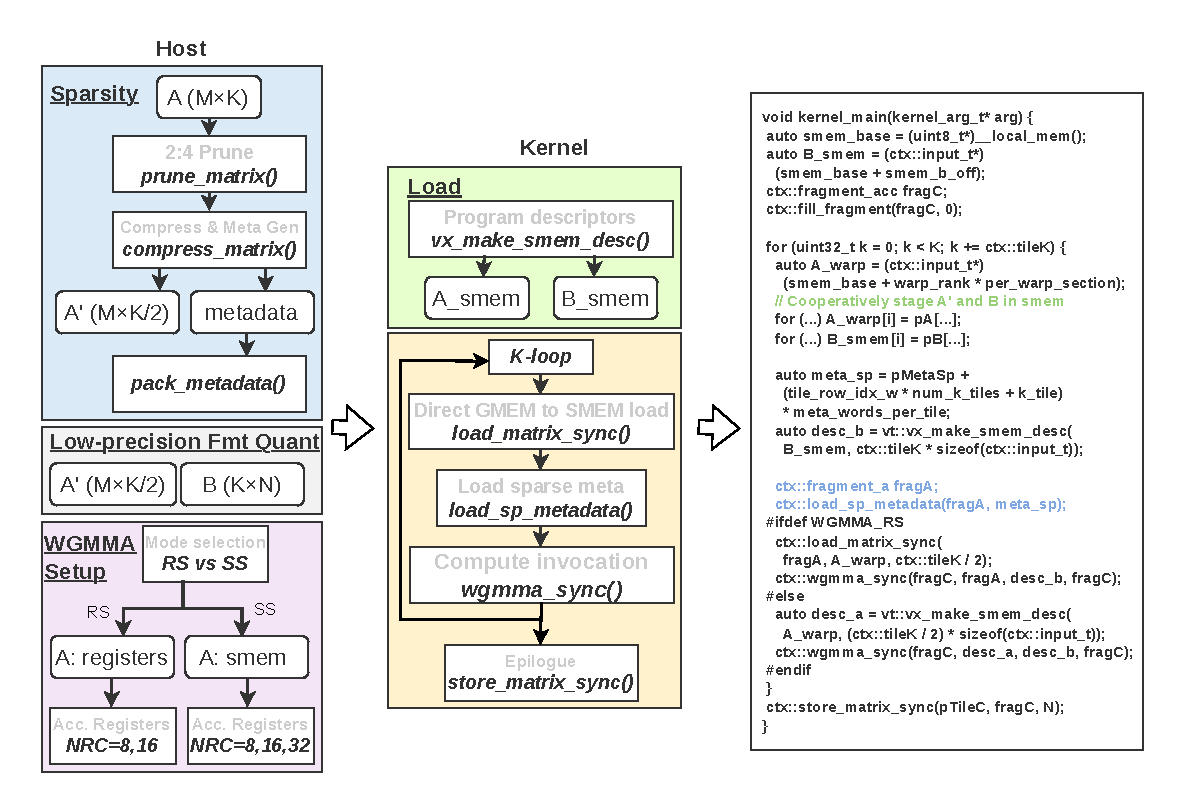
\includegraphics[width=\linewidth]{hpca2027-latex-template/fig/sw_integrationv4.pdf}
    \caption{FourShadow Programming Model}
    \label{fig:sw_integrationv4}
\end{figure}
\label{sec:sw_integrationv4}\label{sec:design_pm}

FourShadow exposes WMMA, WGMMA, and 2:4 structured sparsity as composable primitives selected almost entirely at compile time. Input/output format, NRC, and RS-versus-SS mode are all template parameters on \texttt{wgmma\_config\_t} and \texttt{wgmma\_context} (Figure~\ref{fig:sw_integrationv4}), so the same kernel source compiles down to dense WMMA, dense WGMMA, or sparse WGMMA execution depending on how it is instantiated.

\subsubsection{Host-Side Data Preparation}

\textbf{Metadata Packing.} The 2:4 mask produced by pruning/compression is not uploaded as-is; \texttt{pack\_metadata\_wg} repacks it into the per-thread SRAM bank layout the TCU\_LD AGU and metadata SRAM expect. That layout is dimensioned against the \emph{WMMA}-config per-warp depth since the TCU\_LD path and metadata SRAM are shared hardware sized for WMMA.

\textbf{Compile-Time Mode Selection.} RS keeps $A$ in a register fragment and supports NRC $\le 16$, since the register budget is shared with the $A$ fragment; SS sources both $A$ and $B$ from shared-memory descriptors and supports the full NRC $\in\{8,16,32\}$ range. Both RS/SS and format (\texttt{ITYPE}/\texttt{OTYPE}) are template parameters, fixed at build time.

\subsubsection{Kernel-Side Orchestration}

\textbf{Tile Stride.} Each warp's private $A$ section is padded to the SMEM bank-row width ($\mathit{NT}\times\mathrm{XLEN}/8$ bytes) so warp $w{+}1$'s stripe always starts on a fresh bank row. Without this, the $A$ buffer's single-row fetch can walk into the previous warp's region.

\textbf{Sparse Metadata and Descriptor Dispatch.} Unlike $A$ and $B$, the packed sparse mask bypasses shared memory entirely: \texttt{load\_sp\_metadata} reads it straight from global memory into the TCU's metadata SRAM before dispatch, in both RS and SS mode. The two modes then diverge only in how $A$ reaches the instruction, register fragment via \texttt{load\_matrix\_sync} for RS, shared-memory descriptor via \texttt{vx\_make\_smem\_desc} for SS, but both call the same \texttt{wgmma\_sync} entry point. Sparsity itself is selected once, at compile time, by instantiating \texttt{wgmma\_context} with its sparse flag set, not by a differently named sparse instruction per launch.